Given that our algorithm does not need to maintain stability, we are able to further optimize as compared to a deferred acceptance approach (the one used for hospital residents).  Our algorithm is shown to measurably improve placement at each incremental preference level. The improvements are even more notable when compared to the current non-algorithmic matching effort conducted by humans with imperfect information and an overwhelming amount of data.  

\begin{center}
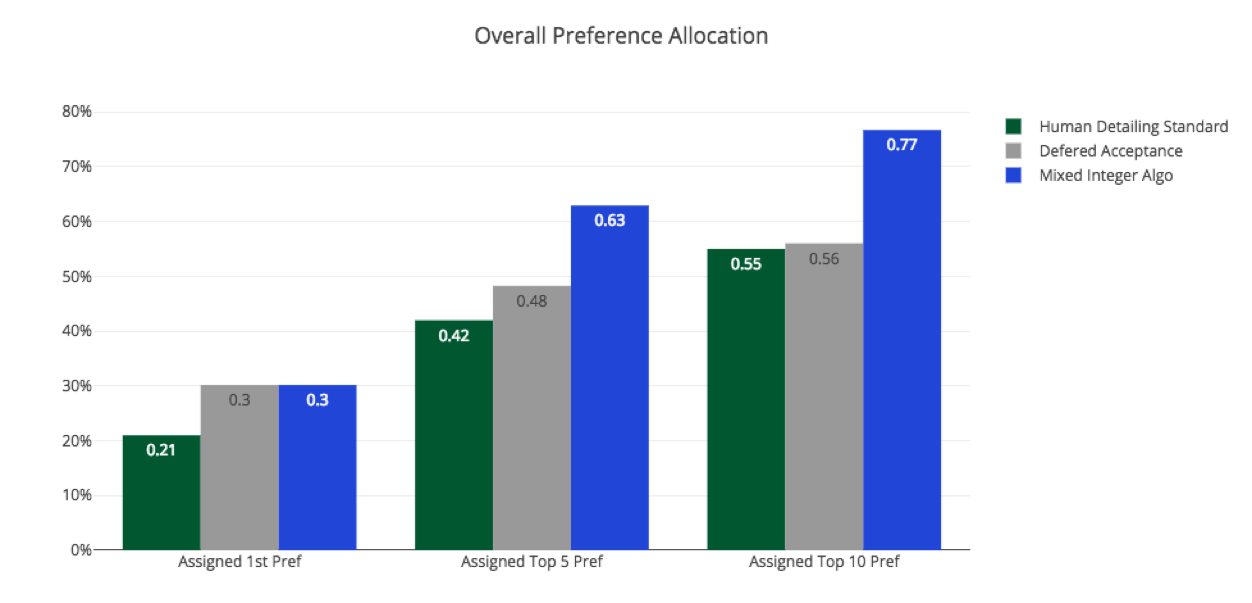
\includegraphics[scale=0.75]{Sections/figures/med_bar.png}
\end{center}

Above is the plot for the Medical Corp data, the plots for all our data sets can be found in Appendix (REF APPENDIX).

%As the below table shows, our algorithm performed better than deferred acceptance across squared average ranking. We chose squared average ranking as the comparative metric due to the view that in the markets we considered the desirability of a position decreases exponentially down ordinal rankings, not linearly.

%[Table]
